% ===================================================================
% Week 03 -- Dynamics and Coding in the Brain (HUJI 769001)
% Lecture 3: attractors and bistability of the autapse (end of sec. 2.3.1), mutual
% inhibition (sec. 2.3.2) and the excitatory-inhibitory pair (sec. 2.3.3). The lecture
% stopped before sec. 2.3.4 (homogeneous all-to-all connectivity).
% No bonus-hour or TA material this week.
% Reference: Loewenstein, Mongillo, Landau & Fox, The Dynamics of Computation in
% Neuronal Networks (../tcns_book-88.pdf), sec. 2.3.1-2.3.3.
% Build: pdflatex -interaction=nonstopmode week03.tex  (twice)
% ===================================================================
% ===================================================================
% Preamble for the Dynamics and Coding in the Brain weekly notes (copy of the shared
% lecture-notes preamble, kept here so this folder builds on its own).
% ===================================================================
\documentclass[11pt,a4paper]{article}

% ---------- encoding & fonts ----------
\usepackage[T1]{fontenc}
\usepackage[utf8]{inputenc}
\usepackage{lmodern}
\renewcommand{\familydefault}{\rmdefault}
\usepackage{microtype}

% ---------- layout ----------
\usepackage[a4paper,margin=2.3cm,top=2.4cm,bottom=2.6cm,headsep=0.9cm]{geometry}
\setlength{\parindent}{0pt}
\setlength{\parskip}{0.55em}
\usepackage{needspace}
\usepackage{multicol}
\usepackage[shortlabels]{enumitem}
\usepackage{array,booktabs,colortbl,tabularx}
\newcolumntype{L}[1]{>{\raggedright\arraybackslash}p{#1}}

% ---------- maths ----------
\usepackage{amsmath,amssymb,mathtools}

% ---------- colours ----------
\usepackage[dvipsnames]{xcolor}
\definecolor{paper}{HTML}{EFE9DA}
\definecolor{surface}{HTML}{FDFBF4}
\definecolor{surface2}{HTML}{F1EBDB}
\definecolor{ink}{HTML}{221C35}
\definecolor{muted}{HTML}{6E6883}
\definecolor{border}{HTML}{4B3C8E}
\definecolor{shadowcol}{HTML}{2E2552}
\definecolor{pgreen}{HTML}{1D6A3B}
\definecolor{ppink}{HTML}{D0307A}
\definecolor{pgold}{HTML}{8C5C0B}
\definecolor{pcyan}{HTML}{2B5FA8}
\pagecolor{paper}
\color{ink}

% ---------- graphics ----------
\usepackage{tikz}
\usetikzlibrary{positioning,arrows.meta,calc,shapes.geometric,shapes.misc,decorations.pathreplacing,patterns,fit,backgrounds}
\usepackage{pgfplots}
\pgfplotsset{compat=1.18}
\tikzset{
  lbl/.style={font=\footnotesize,text=ink,inner sep=1pt},
  blk/.style={draw=ink,line width=1pt,fill=surface,font=\sffamily\scriptsize\bfseries,align=center,minimum height=0.85cm,inner sep=4pt},
  arr/.style={-{Stealth},line width=1.1pt,ink},
  dot/.style={circle,fill=ink,inner sep=1.4pt},
  plbl/.style={font=\ttfamily\scriptsize,text=muted,inner sep=1pt},
  >={Stealth[length=2.6mm]}
}

% ---------- inline semantic markup ----------
\newcommand{\term}[1]{\textcolor{pgreen}{#1}}   % newly defined term
\newcommand{\key}[1]{\textcolor{pcyan}{#1}}     % key word / unit
\newcommand{\hl}[1]{\textcolor{ppink}{#1}}      % the thing to remember
\newcommand{\thd}[1]{{\color{surface}\sffamily\bfseries\footnotesize #1}} % table header cell
\newcommand{\src}[1]{{\ttfamily\scriptsize\textcolor{muted}{[#1]}}}

% ---------- boxes ----------
\usepackage[most]{tcolorbox}
\tcbset{
  notebase/.style={
    enhanced jigsaw, breakable, sharp corners,
    colback=surface, colframe=border, boxrule=1.1pt,
    left=6pt,right=6pt,top=5pt,bottom=5pt,
    before skip=1.1em, after skip=1.1em,
    shadow={1.4mm}{-1.4mm}{0mm}{fill=shadowcol},
    fonttitle=\ttfamily\scriptsize,
    attach boxed title to top left={xshift=3mm,yshift*=-2.4mm},
    boxed title style={sharp corners,boxrule=0.9pt,colframe=surface,
      left=4pt,right=4pt,top=2.5pt,bottom=2.5pt,
      shadow={0.8mm}{-0.8mm}{0mm}{fill=shadowcol}},
    parbox=false,
    before upper={\setlength{\parskip}{0.45em}},
  }
}
\newcommand{\boxtitle}[2]{\if\relax\detokenize{#2}\relax #1\else #1 \textperiodcentered\ \MakeUppercase{#2}\fi}
\newcommand{\boxtitleonly}[2]{\if\relax\detokenize{#2}\relax #1\else \MakeUppercase{#2}\fi}

\newtcolorbox{defn}[1][]{notebase,colbacktitle=pgreen,title={\boxtitle{DEF}{#1}}}
\newtcolorbox{formula}[1][]{notebase,colbacktitle=border,title={\boxtitleonly{FORMULA}{#1}}}
\newtcolorbox{intuition}[1][]{notebase,colbacktitle=ppink,title={\boxtitleonly{KEY IDEA}{#1}}}
\newtcolorbox{example}[1][]{notebase,colbacktitle=pcyan,title={\boxtitle{EXAMPLE}{#1}}}
\newtcolorbox{pitfall}[1][]{notebase,colbacktitle=pgold,title={\boxtitle{PITFALL}{#1}}}
\newtcolorbox{plainbox}{notebase}

% lists inside notes
\setlist[itemize]{label={\textcolor{pgreen}{\scriptsize$\blacksquare$}},leftmargin=1.3em,itemsep=0.25em,topsep=0.3em}
\setlist[enumerate]{label={\textcolor{pgreen}{\ttfamily\arabic*.}},leftmargin=1.6em,itemsep=0.3em,topsep=0.3em}

% ---------- headings ----------
\usepackage{titlesec}
\newcommand{\twodigit}[1]{\ifnum#1<10 0\fi\number#1}
\titleformat{\section}[display]
  {\sffamily\bfseries\fontsize{20}{24}\selectfont\color{pgold}}
  {\ttfamily\small\mdseries\color{pgreen}SECTION \twodigit{\value{section}}}
  {8pt}{}[\vspace{4pt}{\color{border}\titlerule[1.4pt]}]
\titlespacing*{\section}{0pt}{1.6em}{1.0em}
\titleformat{\subsection}
  {\ttfamily\large\color{pcyan}}{>\,\thesubsection}{0.6em}{}
\titlespacing*{\subsection}{0pt}{1.3em}{0.5em}
\titleformat{\subsubsection}
  {\sffamily\bfseries\color{border}}{\thesubsubsection}{0.6em}{}
\titlespacing*{\subsubsection}{0pt}{1.0em}{0.3em}

% ---------- running header / footer ----------
\usepackage{fancyhdr}
\newcommand{\headleft}{}
\newcommand{\headright}{}
\pagestyle{fancy}
\fancyhf{}
\renewcommand{\headrulewidth}{0pt}
\fancyhead[L]{\ttfamily\scriptsize\textcolor{muted}{\headleft}}
\fancyhead[R]{\ttfamily\scriptsize\textcolor{muted}{\headright}}
\fancyfoot[C]{\tikz{\node[draw=border,line width=1pt,fill=surface,inner sep=2.5pt,font=\sffamily\footnotesize] (p) {\thepage};
  \draw[shadowcol,line width=1.6pt] ([yshift=-2pt]p.south west)--([yshift=-2pt]p.south east);}}
\fancypagestyle{plain}{\fancyhf{}\renewcommand{\headrulewidth}{0pt}\fancyfoot[C]{\tikz{\node[draw=border,line width=1pt,fill=surface,inner sep=2.5pt,font=\sffamily\footnotesize] (p) {\thepage};
  \draw[shadowcol,line width=1.6pt] ([yshift=-2pt]p.south west)--([yshift=-2pt]p.south east);}}}

% ---------- links ----------
\usepackage[hidelinks]{hyperref}

\renewcommand{\headleft}{769001 \textperiodcentered\ WEEK 03}
\renewcommand{\headright}{DYNAMICS AND CODING IN THE BRAIN}

\newcommand{\figcap}[1]{\par\smallskip{\small\color{muted}#1}\par}
\newcommand{\hext}{h^{\text{ext}}}
\newcommand{\dr}{\delta r}
\newcommand{\E}{\mathrm{E}}
\newcommand{\I}{\mathrm{I}}
\newcommand{\Tr}{\operatorname{tr}}
\newcommand{\parttitle}[2]{%
  \clearpage
  {\ttfamily\small\color{pgreen}#1}\par\vspace{2pt}
  {\sffamily\bfseries\fontsize{26}{30}\selectfont\color{pgold}#2}\par
  \vspace{4pt}{\color{border}\rule{\linewidth}{1.8pt}}\par\vspace{0.6em}%
  \addtocontents{toc}{\protect\tocpart{#1}}}
\newcommand{\tocpart}[1]{\par\smallskip{\ttfamily\scriptsize\color{pgreen}#1}\par}

\graphicspath{{figures/week03/}}

\begin{document}

% ---------------- title block ----------------
{\ttfamily\small\color{pgreen}HUJI \textperiodcentered\ 769001 \textperiodcentered\ DYNAMICS AND CODING IN THE BRAIN}\par\vspace{6pt}
{\sffamily\bfseries\fontsize{30}{34}\selectfont\color{pgold}Week 03}\par\vspace{4pt}
{\sffamily\bfseries\Large\color{pgold}Attractors, Competition and Oscillations}\par\vspace{4pt}
{\ttfamily\small\color{pcyan}attractor \textperiodcentered\ bistability \textperiodcentered\ memory \textperiodcentered\ mutual inhibition \textperiodcentered\ Jacobian \textperiodcentered\ network modes \textperiodcentered\ pitchfork \textperiodcentered\ symmetry breaking \textperiodcentered\ basin of attraction \textperiodcentered\ decision making \textperiodcentered\ E--I network \textperiodcentered\ Hopf \textperiodcentered\ limit cycle}\par
\vspace{0.8em}

\begin{plainbox}
\textbf{What this week contains.} Part A is Lecture 3, written up from the lecture and the course book \src{LMLF \S2.3.1--2.3.3}. It runs from attractors and bistability of the autapse
(where Week 2 stopped), through two neurons that inhibit each other, to an excitatory--inhibitory pair that oscillates. The lecture stopped just before \S2.3.4 (all-to-all networks).
There was no bonus-hour or TA material this week. Practice problems with full solutions and a cheat sheet close the week.
Errors and typos in the book are corrected in pitfall boxes.
\end{plainbox}

{\ttfamily\small\color{pgreen}CONTENTS}
\begin{multicols}{2}\footnotesize\setlength{\parskip}{0pt}
\setcounter{tocdepth}{1}
\makeatletter\@starttoc{toc}\makeatother
\end{multicols}

% =================================================================
\parttitle{PART A \textperiodcentered\ LECTURE 3 (BOOK \S2.3.1--2.3.3)}{Attractors, Competition and Oscillations}
% =================================================================

\section{Where we are}

Week 2 studied the \term{autapse}: one neuron with a synapse onto itself, of strength $J$ \src{LMLF \S2.3.1}:
\[ \tau\dot r = -r + g(Jr+\hext),\qquad g(x)=\frac{1}{1+e^{-\beta(x-\theta)}}. \]
What we know about it:
\begin{itemize}
  \item A \textbf{fixed point} $r^*$ solves $r^*=g(Jr^*+\hext)$: it is where the S-curve $g(Jr+\hext)$ crosses the identity line.
  \item Its \textbf{stability} is set by $\lambda = Jg'(Jr^*+\hext)$, the slope of the S-curve at the crossing: $\lambda<1$ stable, $\lambda>1$ unstable.
  \item With the book's values $\theta=0$, $\beta=20$, $J=1$: for $-0.803<\hext<-0.197$ there are three fixed points, otherwise one. At the two edges a stable and an unstable fixed point merge and vanish: a \textbf{saddle-node bifurcation}.
\end{itemize}

\begin{intuition}[The plan for this week: three tiny networks, three behaviours]
\begin{enumerate}
  \item \textbf{One excitatory neuron} (the autapse): two stable states, so it can \hl{remember a bit}.
  \item \textbf{Two neurons that inhibit each other}: one wins and silences the other, so they can \hl{make a decision}.
  \item \textbf{One excitatory and one inhibitory neuron}: neither settles down, so they \hl{oscillate}.
\end{enumerate}
The tools are the same every time: find the fixed points, linearize around them, read stability from the eigenvalues. In two dimensions the single number $\lambda$ becomes a $2\times2$ matrix, and Week 1's eigenvalue tools take over.
\end{intuition}

% =================================================================
\section{Attractors and bistability}

\subsection{Attractors and bistability}

\begin{defn}[State space and attractor]
The \term{state space} is the set of all possible states of the system; for the autapse it is just the $r$ axis.
An \term{attractor} is a region of state space to which all nearby trajectories converge \src{LMLF 2.3.1}. A stable fixed point is the simplest attractor; this week we will meet another kind, the limit cycle (\S\ref{sec:limitcycle}).
\end{defn}

\begin{defn}[Bistability]
A system is \term{bistable} if it has \hl{two stable fixed points} (two attractors). Between them there is always an unstable fixed point, which separates the starting values that go to one from those that go to the other.
The autapse is bistable for $-0.803<\hext<-0.197$ (with $\theta=0$, $\beta=20$, $J=1$).
\end{defn}

\begin{example}[Where does the neuron end up? ($\hext=-0.5$, $\tau=10$\,ms)]
\begin{center}
\renewcommand{\arraystretch}{1.2}
\begin{tabular}{c|ccccccc}
$t$ (ms) & 0 & 10 & 20 & 30 & 50 & 70 & 100\\\hline
$r(0)=0.40$ & 0.40 & 0.157 & 0.058 & 0.021 & 0.003 & 0.000 & 0.000\\
$r(0)=0.45$ & 0.45 & 0.194 & 0.072 & 0.026 & 0.004 & 0.001 & 0.000\\
$r(0)=0.55$ & 0.55 & 0.806 & 0.928 & 0.974 & 0.996 & 0.999 & 1.000\\
$r(0)=0.60$ & 0.60 & 0.843 & 0.942 & 0.979 & 0.997 & 1.000 & 1.000\\
\end{tabular}
\end{center}
(Numerical solutions.) Starting values only $0.1$ apart end in opposite states. The final state is decided entirely by \hl{which side of $0.5$} the neuron starts on: $0.5$ is the unstable fixed point.
\end{example}

\begin{pitfall}[Three intersections, not two]
The book says that the bistable regime has ``two intersection points''. It has \emph{three} intersections (fixed points), of which \emph{two} are stable. The unstable middle one is always there, between the two attractors.
\end{pitfall}

\subsection{Memory: switching with a brief input}

Why care about two stable states? Because a bistable neuron can \hl{store one bit} \src{LMLF 2.3.1}. Left alone in the bistable range, it stays forever in whichever state it is in.
To write a bit, change $\hext$ \emph{briefly}:

\begin{enumerate}
  \item The neuron rests in the low state, $\hext=-0.5$.
  \item A brief pulse raises $\hext$ to $0$, \emph{above} the bifurcation point $-0.197$. Now the low fixed point no longer exists; the only attractor is the high one, and $r$ starts climbing.
  \item The pulse ends: $\hext$ returns to $-0.5$. The low state exists again, but if $r$ has already passed the watershed $0.5$, it keeps going to the high state.
  \item The neuron stays high indefinitely, although the input that put it there is long gone. That is memory.
  \item To erase, pulse $\hext$ \emph{below} $-0.803$ (here to $-1$): the high state disappears and the neuron falls back to the low one, where it stays.
\end{enumerate}

\begin{center}
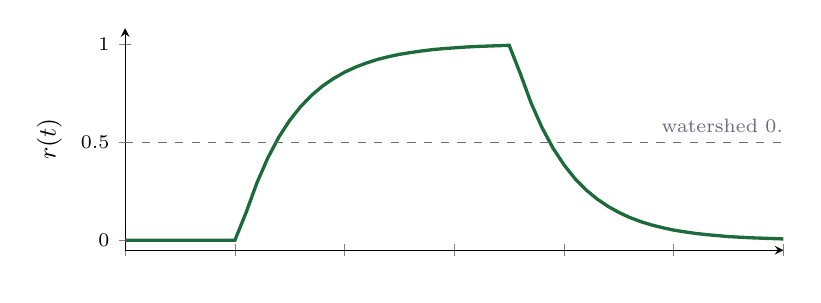
\begin{tikzpicture}
\begin{axis}[width=0.82\linewidth,height=4.4cm,xmin=0,xmax=120,ymin=-0.05,ymax=1.08,
  ylabel={$r(t)$},axis lines=left,tick label style={font=\scriptsize},label style={font=\small},xticklabels={}]
  \addplot[pgreen,very thick] coordinates {(0,0.000) (2,0.000) (4,0.000) (6,0.000) (8,0.000) (10,0.000) (12,0.000) (14,0.000) (16,0.000) (18,0.000) (20,0.000) (22,0.138) (24,0.291) (26,0.419) (28,0.525) (30,0.611) (32,0.681) (34,0.739) (36,0.786) (38,0.824) (40,0.856) (42,0.882) (44,0.903) (46,0.921) (48,0.935) (50,0.947) (52,0.956) (54,0.964) (56,0.971) (58,0.976) (60,0.980) (62,0.984) (64,0.987) (66,0.989) (68,0.991) (70,0.993) (72,0.851) (74,0.699) (76,0.573) (78,0.469) (80,0.384) (82,0.314) (84,0.257) (86,0.211) (88,0.173) (90,0.142) (92,0.116) (94,0.095) (96,0.078) (98,0.064) (100,0.052) (102,0.043) (104,0.035) (106,0.029) (108,0.024) (110,0.019) (112,0.016) (114,0.013) (116,0.011) (118,0.009) (120,0.007)};
  \addplot[muted,dashed] coordinates {(0,0.5) (120,0.5)};
  \node[font=\scriptsize,muted,anchor=south west] at (axis cs:96,0.5) {watershed $0.5$};
\end{axis}
\end{tikzpicture}

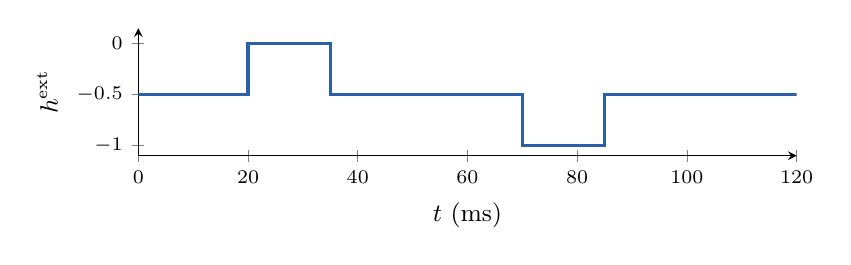
\begin{tikzpicture}
\begin{axis}[width=0.82\linewidth,height=3.2cm,xmin=0,xmax=120,ymin=-1.1,ymax=0.15,
  xlabel={$t$ (ms)},ylabel={$\hext$},axis lines=left,tick label style={font=\scriptsize},label style={font=\small},ytick={-1,-0.5,0}]
  \addplot[pcyan,very thick] coordinates {(0,-0.5) (20,-0.5) (20,0) (35,0) (35,-0.5) (70,-0.5) (70,-1) (85,-1) (85,-0.5) (120,-0.5)};
\end{axis}
\end{tikzpicture}
\figcap{State transitions, simulated after \src{LMLF Fig.\ 2.9} ($\theta=0$, $\beta=20$, $J=1$, $\tau=10$\,ms). A 15\,ms pulse to $\hext=0$ switches the neuron on (it has reached $0.76>0.5$ when the pulse ends);
a 15\,ms pulse to $\hext=-1$ switches it off (it has fallen to $0.23<0.5$). In between, at the same $\hext=-0.5$, the neuron is high or low depending only on its history.}
\end{center}

\begin{intuition}[The state depends on history]
At $t=10$\,ms and at $t=60$\,ms the input is the same, $\hext=-0.5$, but the rate is $0$ in one case and $0.98$ in the other. The difference is \hl{what happened before}.
This dependence on past input (often called \term{hysteresis}) is what lets a single neuron with feedback hold information; the book develops it into a model of long-term memory in Ch.\ 5.
\end{intuition}

\begin{pitfall}[The pulse must be long enough]
Raising $\hext$ is not enough by itself; the rate must cross the watershed $0.5$ \emph{before} the pulse ends. With the same parameters, a 5\,ms pulse to $\hext=0$ brings $r$ only to $0.36$.
When $\hext$ returns to $-0.5$, the rate is on the low side of $0.5$ and decays back to $0$: nothing is stored.
\end{pitfall}

\subsection{The two ingredients: positive feedback and saturation}\label{sec:ingredients}

What makes bistability possible? We need an S-curve that can cross the identity line three times. Two things are required \src{LMLF 2.3.1}:
\begin{itemize}
  \item \textbf{Positive feedback} that is strong enough: in the middle crossing the S-curve must be steeper than $1$. Its maximal slope is $\beta J/4$ (the effective gain over $4$), so we need
        \[ \boxed{\ \frac{\beta J}{4} > 1\ }. \]
        If this fails, the S-curve is flatter than the identity line everywhere and crosses it only once, whatever $\hext$ is. If it holds, a suitable $\hext$ produces three crossings.
  \item \textbf{Saturation}: the curve must bend back below the identity line at high $r$ (and stay above it at low $r$). That is what the bounded logistic function provides,
        and what the linear $g$ lacked: there, $J>1$ meant an unstable fixed point and divergence, with no second stable state to land in.
\end{itemize}

\begin{example}[How much feedback is enough? ($\beta=20$)]
$\beta J/4 > 1 \iff J > 4/\beta = 0.2$. With the book's $J=1$: $\beta J/4 = 5$, comfortably bistable for some range of $\hext$. With $J=0.1$: $\beta J/4 = 0.5$, one fixed point for every $\hext$, no memory.
\end{example}

Keep these two ingredients in mind: we will meet them again in the next network, where the positive feedback comes, surprisingly, from inhibition (\S\ref{sec:disinhibition}).

\subsection{A technical aside: the case $\lambda = 1$}

The linearization decides stability whenever $\lambda\neq1$. When $\lambda=1$ exactly, it gives $\tau\dot{\dr}=0$, which says nothing. This happens precisely at the bifurcation points, where the S-curve is tangent to the identity line.

\textbf{Step 1: expand one order further} \src{LMLF eq.\ 2.23--2.25}. A second-order Taylor expansion adds the curvature term:
\[ g(h^*+J\dr) \approx g(h^*) + g'(h^*)J\dr + \tfrac12 g''(h^*)J^2\dr^2. \]
\textbf{Step 2: substitute}. The constant term vanishes (fixed point) and the linear term vanishes ($\lambda=1$), leaving
\[ \tau\,\dot{\dr} = \tfrac12 J^2 g''(h^*)\,\dr^2. \]
\textbf{Step 3: read the sign.} $\dr^2>0$ on \emph{both} sides of $r^*$, so $\dot{\dr}$ has the same sign (that of $g''$) on both sides. The flow goes towards $r^*$ on one side and away on the other.

\begin{defn}[Half-stable fixed point]
A fixed point is \term{half-stable} if the dynamics approach it from one side and leave it on the other.
\end{defn}

\textbf{Step 4: solve} (the equation is separable): $\displaystyle\frac{d\dr}{\dr^2} = c\,dt$ with $c = \frac{J^2g''(h^*)}{2\tau}$, so $-\frac{1}{\dr} = ct + \text{const}$ and
\[ \dr(t) = \frac{1}{1/\dr(0) - c\,t}. \]
This is \term{hyperbolic}, not exponential: much slower near the fixed point.

\begin{example}[At the bifurcation point $\hext=-0.803$ ($\beta=20$, $J=1$, $\tau=10$\,ms)]
Here $r^*=0.947$, and $g'' = \beta^2 g(1-g)(1-2g) = 400\cdot0.947\cdot0.053\cdot(-0.894) = -17.9$, so $c = -17.9/20 = -0.89$ per ms.
\begin{itemize}
  \item From above, $\dr(0)=+0.01$: $\dr(t) = 1/(100+0.89t)$. After $100$\,ms it is $0.0053$: only halved. (An exponential decay with $\tau=10$\,ms would have shrunk it $e^{10}\approx 22\,000$-fold.)
  \item From below, $\dr(0)=-0.01$: $\dr(t) = 1/(-100+0.89t)$ grows in size and the approximation breaks down after about $100$\,ms; the neuron leaves towards the low state.
\end{itemize}
\end{example}

\begin{pitfall}[Linearization tells you only about the neighbourhood]
Both the first- and second-order expansions are valid only while $\dr$ is small. They decide \emph{local} stability. Whether a fixed point is reached from far away (global stability) needs the full picture, such as the vector field \src{LMLF 2.3.1}.
And $\lambda=1$ exactly is a knife-edge: the slightest change of $\hext$ makes $\lambda\neq1$, and the exponential behaviour takes over again.
\end{pitfall}

% =================================================================
\section{Mutual inhibition: the model}

After one neuron, the next simplest network has two \src{LMLF \S2.3.2}.

\begin{defn}[Mutual inhibition]
Two neurons (or two populations) are in \term{mutual inhibition} if each one inhibits the other. Here the inhibition is \term{symmetric}: both synapses have the same strength $J>0$.
\end{defn}

\begin{center}
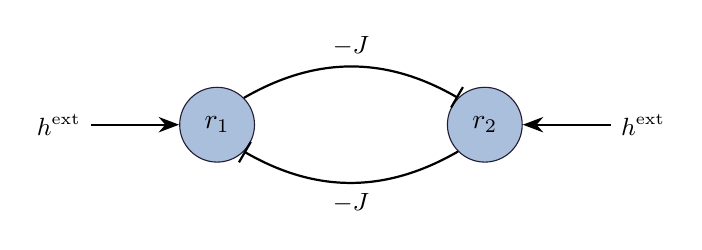
\begin{tikzpicture}
  \node[draw=ink,fill=pcyan!40,circle,minimum size=0.95cm,font=\sffamily\bfseries] (A) at (0,0) {$r_1$};
  \node[draw=ink,fill=pcyan!40,circle,minimum size=0.95cm,font=\sffamily\bfseries] (B) at (3.4,0) {$r_2$};
  \draw[thick,-{Bar[width=3mm]}] (A.north east) to[bend left=30] node[above,font=\small]{$-J$} (B.north west);
  \draw[thick,-{Bar[width=3mm]}] (B.south west) to[bend left=30] node[below,font=\small]{$-J$} (A.south east);
  \draw[thick,->] (-1.6,0) node[left,font=\small]{$\hext$} -- (A.west);
  \draw[thick,->] (5.0,0) node[right,font=\small]{$\hext$} -- (B.east);
\end{tikzpicture}
\figcap{Two neurons inhibiting each other, redrawn after \src{LMLF Fig.\ 2.10}. A flat bar at the end of a connection means inhibition. Both neurons get the same external input $\hext$.}
\end{center}

The rate equations, with time measured in units of $\tau$ (so $\tau=1$) and $g$ the logistic function \src{LMLF eq.\ 2.29}:
\[ \boxed{\ \dot r_1 = -r_1 + g(-Jr_2+\hext),\qquad \dot r_2 = -r_2 + g(-Jr_1+\hext)\ } \]
\begin{itemize}
  \item Neuron $1$ hears neuron $2$ through the term $-Jr_2$. Since $J>0$, the \emph{minus} sign makes the synapse inhibitory: the more neuron $2$ fires, the smaller neuron $1$'s input.
  \item There are no self-connections: neuron $1$'s input does not contain $r_1$.
  \item Both neurons get the same external input $\hext$. That makes the two neurons interchangeable, a symmetry that will matter.
\end{itemize}

\begin{pitfall}[Where is the inhibition?]
The inhibition is the \emph{sign in front of} $J$, not the sign of $J$. The book takes $J>0$ and writes $-J$ explicitly. Do not also make $J$ negative: $-(-J)r_2$ would be excitation.
\end{pitfall}

\section{The homogeneous fixed point}

\subsection{The symmetric solution}

The fixed points solve $\dot r_1=\dot r_2=0$:
\[ r_1^* = g(-Jr_2^*+\hext),\qquad r_2^* = g(-Jr_1^*+\hext). \]
Swap the names $1\leftrightarrow2$: the pair of equations is unchanged. So it is natural to look for a solution that is unchanged too, with both neurons firing at the same rate.

\begin{defn}[Homogeneous fixed point]
A fixed point is \term{homogeneous} if all neurons have the same rate, $r_1^*=r_2^*=r^*$. For mutual inhibition it solves
\[ r^* = g(-Jr^*+\hext)\qquad\text{\src{LMLF eq.\ 2.32}}. \]
\end{defn}

\subsection{There is always exactly one}

The equation $r^*=g(-Jr^*+\hext)$ has exactly one solution, for every $J>0$ and every $\hext$. The argument, step by step:
\begin{enumerate}
  \item Compare the left side $L(r)=r$ with the right side $R(r)=g(-Jr+\hext)$ on $0\le r\le1$ (the logistic $g$ is always between $0$ and $1$).
  \item At $r=0$: $L=0$ and $R=g(\hext)>0$. So $R>L$.
  \item At $r=1$: $L=1$ and $R=g(-J+\hext)<1$. So $R<L$.
  \item $L$ is increasing. $R$ is \emph{decreasing}, because a larger $r$ means more inhibition, hence less input, hence a smaller $g$.
  \item A continuous curve that starts above and ends below must cross at least once; an increasing and a decreasing curve can cross at most once. So: \hl{exactly one crossing}.
\end{enumerate}

\begin{intuition}[Compare with the autapse]
In the excitatory autapse the right side $g(Jr+\hext)$ was \emph{increasing}, an S-curve that could cross the identity line three times. Inhibition flips it into a falling curve, which can cross only once.
So the \emph{homogeneous} equation never has more than one solution. If bistability appears, it must come from \emph{non-homogeneous} fixed points, with $r_1^*\neq r_2^*$. That is exactly what will happen.
\end{intuition}

\begin{example}[The book's Fig.\ 2.11 parameters: $\theta=0$, $\beta=5$, $J=2$, $\hext=1$]
Try $r^*=0.5$: the input is $-2(0.5)+1=0$, and $g(0)=0.5$ \checkmark. So $r^*=0.5$ exactly, with input $h^*=0$.
\end{example}

\begin{example}[The book's Fig.\ 2.12 parameters: $\theta=0$, $\beta=1$, $\hext=1$, $J=3$]
No guess works exactly, so iterate or bisect: $r^*=0.4288$. Check: input $h^*=-3(0.4288)+1=-0.286$, and $g(-0.286)=1/(1+e^{0.286})=0.429$ \checkmark.
\end{example}

\section{Linearizing: the Jacobian}

\subsection{Perturbing two neurons}

Is the homogeneous fixed point stable? As in Week 2, nudge the state slightly and see whether the nudge shrinks or grows. The new feature: there are now \hl{two} numbers to nudge, and nudging one affects the other.

Write $r_i(t)=r^*+\dr_i(t)$ for $i=1,2$, and call $h^*=-Jr^*+\hext$ the input at the fixed point. Step by step for neuron $1$:
\begin{enumerate}
  \item Substitute: $\frac{d}{dt}(r^*+\dr_1) = -(r^*+\dr_1) + g\big(-J(r^*+\dr_2)+\hext\big) = -r^*-\dr_1+g(h^*-J\dr_2)$.
  \item $r^*$ is a constant, so the left side is just $\dot{\dr}_1$.
  \item First-order Taylor expansion of $g$ around $h^*$: $g(h^*-J\dr_2)\approx g(h^*)+g'(h^*)(-J\dr_2)$.
  \item $-r^*+g(h^*)=0$, because $r^*$ is a fixed point. What is left:
        \[ \dot{\dr}_1 = -\dr_1 - Jg'(h^*)\,\dr_2. \]
  \item Neuron $2$ is the same with $1\leftrightarrow2$: $\dot{\dr}_2 = -\dr_2 - Jg'(h^*)\,\dr_1$.
\end{enumerate}
Call $a\equiv Jg'(h^*)$, the \term{effective coupling} at the fixed point. In matrix form \src{LMLF eq.\ 2.36--2.37}:
\[ \boxed{\ \dot{\vec{\dr}} = M\,\vec{\dr},\qquad M=\begin{pmatrix}-1 & -a\\ -a & -1\end{pmatrix},\qquad a=Jg'(h^*)>0\ } \]
$a>0$ because $J>0$ and the logistic function is increasing ($g'>0$).

\begin{formula}[A shortcut for $g'$ at a fixed point]
For the logistic function $g'=\beta g(1-g)$. At the fixed point $g(h^*)=r^*$, so
\[ g'(h^*)=\beta r^*(1-r^*),\qquad a=\beta J\,r^*(1-r^*). \]
No exponentials needed once $r^*$ is known. Example ($\beta=1$, $J=3$, $r^*=0.4288$): $a=3\cdot0.4288\cdot0.5712=0.735$.
\end{formula}

\subsection{The Jacobian}

\begin{defn}[Jacobian matrix]
Write the dynamics as $\dot{\vec r}=\vec F(\vec r)$; here $F_1=-r_1+g(-Jr_2+\hext)$ and $F_2=-r_2+g(-Jr_1+\hext)$. The \term{Jacobian} at a point $\vec r^*$ is the matrix of all first partial derivatives,
\[ M_{ij}=\frac{\partial F_i}{\partial r_j}\Big|_{\vec r^*}. \]
Row $i$ says how $\dot r_i$ responds to a small change of each rate. Near a fixed point the dynamics of the perturbation are $\dot{\vec{\dr}}=M\vec{\dr}$: the Jacobian is the many-dimensional version of Week 2's single number $\lambda-1$.
It depends on the point where you evaluate it.
\end{defn}

\begin{example}[The same $M$ from partial derivatives]
$\partial F_1/\partial r_1=-1$ (the leak), $\partial F_1/\partial r_2=g'(\cdot)\cdot(-J)=-Jg'(h^*)=-a$ (chain rule). Likewise $\partial F_2/\partial r_1=-a$ and $\partial F_2/\partial r_2=-1$. This is the matrix above. \checkmark
\end{example}

\begin{intuition}[What the off-diagonal entries do]
The diagonal entries ($-1$, the leak) describe each neuron on its own; the off-diagonal entries ($-a$) are the \hl{coupling}. If $M$ were diagonal, each perturbation would evolve alone, $\dot{\dr}_i=M_{ii}\dr_i$, and the fixed point would be stable iff every $M_{ii}<0$.
Here $M$ is not diagonal: pushing neuron $1$ up pushes neuron $2$ down. We cannot judge stability neuron by neuron. We need directions in which the dynamics \emph{do} decouple: the eigenvectors.
\end{intuition}

\section{Network modes: eigenvectors of the Jacobian}

\subsection{From neurons to modes}

\begin{defn}[Network mode]
A \term{mode} is a fixed pattern of activity across the neurons, given by an eigenvector $\vec u$ of the Jacobian: changing every neuron by the amounts in $\vec u$ \src{LMLF \S2.3.2}.
A perturbation along an eigenvector stays along it, $\vec{\dr}(t)=c(t)\vec u$ with $\dot c=\mu c$, so $c(t)=c(0)e^{\mu t}$. Different modes do \emph{not} affect each other.
\end{defn}

So in the \emph{neuron} basis the variables are coupled, while in the \emph{mode} (eigenvector) basis they are not. A general perturbation is a sum of modes, and each mode grows or decays on its own.

\begin{formula}[Stability from the eigenvalues]
If the eigenvectors of $M$ span the space, every perturbation is a combination of modes, and
\begin{itemize}
  \item all eigenvalues with \textbf{negative real part}: every mode decays, \hl{the fixed point is stable};
  \item at least one eigenvalue with \textbf{positive real part}: that mode grows, \hl{the fixed point is unstable}.
\end{itemize}
For complex eigenvalues only the real part decides (it sets $|e^{\mu t}|=e^{\operatorname{Re}\mu\,t}$); the imaginary part makes the mode rotate. We will need this in the E--I network.
\end{formula}

\subsection{The two modes of mutual inhibition}

Finding the eigenvectors of $M=\begin{pmatrix}-1&-a\\-a&-1\end{pmatrix}$ needs no characteristic polynomial. Two shortcuts from Week 2 Part B do it:
\begin{enumerate}
  \item \textbf{Equal row sums.} Both rows add up to $-1-a$. So $M\mathbf1=-(1+a)\mathbf1$: the vector $\vec u_\parallel=(1,1)$ is an eigenvector with eigenvalue $-(1+a)$.
  \item \textbf{Symmetry.} $M=M^T$, so eigenvectors with different eigenvalues are orthogonal. The other one is perpendicular to $(1,1)$: $\vec u_\perp=(1,-1)$.
  \item \textbf{Check} by multiplying: $M(1,-1)^T=(-1+a,\;-a+1)^T=-(1-a)(1,-1)^T$. Eigenvalue $-(1-a)$.
\end{enumerate}

\begin{formula}[Modes of mutual inhibition \src{LMLF eq.\ 2.37}]
\begin{center}
\renewcommand{\arraystretch}{1.3}
\begin{tabular}{lll}
\textbf{mode} & \textbf{eigenvector} & \textbf{eigenvalue}\\\hline
\term{homogeneous} direction (both neurons together) & $\vec u_\parallel=(1,1)$ & $\mu_\parallel=-(1+a)$\\
\term{heterogeneous} direction (one up, one down) & $\vec u_\perp=(1,-1)$ & $\mu_\perp=-(1-a)$\\
\end{tabular}
\end{center}
\end{formula}

\subsection{The full solution, mode by mode}

This is the decoupling of Week 2 Part B, now with $a=Jg'(h^*)$ coming from the network. Define the sum and difference of the perturbations, $\dr_+=\dr_1+\dr_2$ and $\dr_-=\dr_1-\dr_2$. Adding and subtracting the two equations:
\[ \dot{\dr}_+=-(1+a)\,\dr_+,\qquad \dot{\dr}_-=-(1-a)\,\dr_- . \]
Each is a one-variable equation from Week 1:
\[ \dr_+(t)=\dr_+(0)e^{-(1+a)t},\qquad \dr_-(t)=\dr_-(0)e^{-(1-a)t}, \]
and back to the neurons, $\dr_{1,2}=\tfrac12(\dr_+\pm\dr_-)$:
\[ \boxed{\ \dr_1(t)=\tfrac12\big[\dr_+(0)e^{-(1+a)t}+\dr_-(0)e^{-(1-a)t}\big],\qquad \dr_2(t)=\tfrac12\big[\dr_+(0)e^{-(1+a)t}-\dr_-(0)e^{-(1-a)t}\big]\ } \]

\begin{example}[Kick one neuron: $\beta=1$, $\hext=1$, $J=3$, so $a=0.735$]
Start with $\dr(0)=(0.02,\,0)$: only neuron $1$ is pushed up. Then $\dr_+(0)=\dr_-(0)=0.02$, and $\mu_\parallel=-1.735$, $\mu_\perp=-0.265$.
\begin{center}
\renewcommand{\arraystretch}{1.2}
\begin{tabular}{c|cc|cc}
$t$ & $\dr_+$ & $\dr_-$ & $\dr_1$ & $\dr_2$\\\hline
0 & 0.0200 & 0.0200 & 0.0200 & 0\\
1 & 0.0035 & 0.0153 & 0.0094 & $-0.0059$\\
2 & 0.0006 & 0.0118 & 0.0062 & $-0.0056$\\
4 & 0.0000 & 0.0069 & 0.0035 & $-0.0035$\\
\end{tabular}
\end{center}
Read the table:
\begin{itemize}
  \item Neuron $2$ was not touched, yet it goes \emph{down}: neuron $1$ is now firing more and inhibits it.
  \item The sum $\dr_+$ is gone by $t\approx2$; what remains is a pure difference, $\dr_1\approx-\dr_2$.
  \item The difference decays too, but slowly (rate $0.265$). Both modes decay: the fixed point is stable.
\end{itemize}
\end{example}

\section{When the symmetric state becomes unstable}

\subsection{The stability verdict}

\begin{itemize}
  \item $\mu_\parallel=-(1+a)<0$ \textbf{always}, since $a>0$. The homogeneous fixed point is always stable against perturbations that move both neurons equally.
  \item $\mu_\perp=-(1-a)<0$ \textbf{iff} $a<1$. If the inhibition is strong enough that $a>1$, the heterogeneous mode grows: \hl{the homogeneous fixed point is unstable}, and the direction of instability is $(1,-1)$.
\end{itemize}

\begin{formula}[Stability of the homogeneous state]
\[ \text{stable}\iff a=Jg'(h^*)=\beta J\,r^*(1-r^*)<1. \]
When it fails, two neurons that start with similar but not equal rates move \emph{apart}.
\end{formula}

\begin{example}[Scanning $J$ ($\theta=0$, $\beta=1$, $\hext=1$; the book's Fig.\ 2.12 parameters)]
\begin{center}
\renewcommand{\arraystretch}{1.25}
\begin{tabular}{c|ccc|l}
$J$ & $r^*$ & $a=Jr^*(1-r^*)$ & $\mu_\perp=-(1-a)$ & homogeneous state\\\hline
1 & 0.599 & 0.240 & $-0.760$ & stable\\
3 & 0.429 & 0.735 & $-0.265$ & stable\\
4 & 0.376 & 0.939 & $-0.061$ & stable (barely)\\
4.33 & 0.362 & 1.000 & $0$ & critical\\
5 & 0.336 & 1.116 & $+0.116$ & unstable\\
10 & 0.224 & 1.739 & $+0.739$ & unstable\\
\end{tabular}
\end{center}
As $J$ grows, $r^*$ falls (more inhibition), but $a$ still grows, and crosses $1$ at $J_c\approx4.33$.
\end{example}

\begin{pitfall}[$a$ is not proportional to $J$]
$a=Jg'(h^*)$ depends on $J$ twice: directly, and through $r^*$ (hence $h^*$ and the slope $g'$). So the critical $J$ cannot be read off as ``$J=1/g'$''. It has to be found by solving $r^*=g(-Jr^*+\hext)$ and $Jr^*(1-r^*)=1$ together; here numerically, $J_c\approx4.33$, $r^*\approx0.362$.
A quick bound: $r(1-r)\le\tfrac14$, so with $\beta=1$, $a\le J/4$, and the homogeneous state is stable for every $J<4$, whatever $\hext$ is.
\end{pitfall}

\begin{example}[The Fig.\ 2.11 parameters are already unstable]
With $\beta=5$, $J=2$, $\hext=1$ we found $r^*=0.5$. Then $a=\beta Jr^*(1-r^*)=5\cdot2\cdot0.25=2.5>1$. The homogeneous state there is unstable: the figure shows a fixed point that the network will not stay at.
\end{example}

The input matters too: $a$ depends on the slope $g'(h^*)$, and $h^*$ depends on $\hext$. So changing $\hext$ alone can also destabilize the homogeneous state \src{LMLF \S2.3.2}.

\subsection{Symmetry breaking and the pitchfork}

What does the network do once the homogeneous state is unstable? Because the connectivity is symmetric, the only attractors are fixed points (the book proves this in \S2.4 with an energy function; here we take it as given). New fixed points must appear, and they do.

\begin{defn}[Symmetry breaking]
The equations are unchanged when the two neurons are swapped, but a solution need not be. A fixed point with $r_1^*\neq r_2^*$ \term{breaks the symmetry}.
The symmetry survives only in the \emph{set} of solutions: if $(r_A,r_B)$ is a fixed point, so is $(r_B,r_A)$. They come in mirror pairs.
\end{defn}

\begin{defn}[Pitchfork bifurcation]
A \term{pitchfork bifurcation} is a bifurcation in which one stable fixed point becomes unstable and, at the same moment, \hl{two new stable fixed points branch off from it}, symmetric to each other.
In the bifurcation diagram one line splits into three, like the prongs of a fork. Compare Week 2: in a \emph{saddle-node} bifurcation two fixed points merge and vanish; here none vanish, one changes stability and two are born.
(The $\tanh$ population of TA session 2 had a pitchfork too, at $J=1$.)
\end{defn}

\begin{center}
\fcolorbox{border}{white}{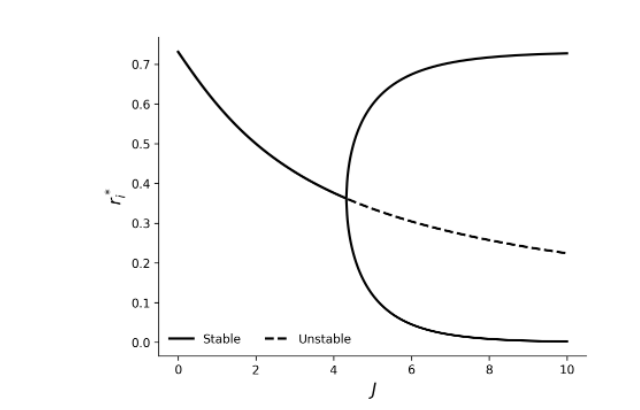
\includegraphics[width=0.62\linewidth]{mutual_inhibition_bifurcation}}
\figcap{\src{LMLF Fig.\ 2.12}. The fixed-point rates $r_i^*$ against $J$ ($\hext=1$, $\beta=1$, $\theta=0$). Solid: stable; dashed: unstable. Left of $J_c\approx4.33$: one homogeneous fixed point, stable.
Right of it: the homogeneous one continues as the dashed line (unstable), and two stable asymmetric fixed points appear. On each of them one neuron is high (upper branch) and the other low (lower branch).}
\end{center}

\begin{example}[The asymmetric fixed points at $J=5$]
Numerically, $(r_1^*,r_2^*)=(0.599,\,0.120)$, and its mirror image $(0.120,\,0.599)$. Check the first:
\begin{itemize}
  \item neuron $1$: input $-5(0.120)+1=0.400$, $g(0.400)=1/(1+e^{-0.4})=0.599$ \checkmark;
  \item neuron $2$: input $-5(0.599)+1=-1.995$, $g(-1.995)=1/(1+e^{1.995})=0.120$ \checkmark.
\end{itemize}
At $J=10$ the asymmetry is stronger: $(0.727,\,0.0019)$. The loser is practically silent.
\end{example}

\begin{example}[Watching one neuron win ($J=5$, start $r(0)=(0.35,\,0.33)$)]
The start is close to the unstable homogeneous point $(0.336,0.336)$, with neuron $1$ slightly ahead. Simulating:
\begin{center}
\renewcommand{\arraystretch}{1.2}
\begin{tabular}{c|cccccccc}
$t$ (units of $\tau$) & 0 & 5 & 10 & 15 & 20 & 25 & 30 & 40\\\hline
$r_1$ & 0.350 & 0.354 & 0.368 & 0.392 & 0.432 & 0.485 & 0.538 & 0.588\\
$r_2$ & 0.330 & 0.319 & 0.305 & 0.282 & 0.247 & 0.203 & 0.163 & 0.127\\
\end{tabular}
\end{center}
The small head start of $0.02$ grows (at first like $e^{+0.116t}$, the rate $\mu_\perp$) until saturation takes over and the state settles at $(0.599,0.120)$. Starting from $(0.33,0.35)$ instead gives the mirror image: neuron $2$ wins.
\end{example}

\subsection{Where does the positive feedback come from? Disinhibition}\label{sec:disinhibition}

In \S\ref{sec:ingredients} we said bistability needs positive feedback and saturation. The saturation is the logistic $g$ again. But every synapse here is \emph{inhibitory}: where is the positive feedback?

\begin{defn}[Disinhibition]
\term{Disinhibition} is the removal of inhibition: inhibiting an inhibitory neuron reduces the inhibition it sends out, which \emph{excites} its targets indirectly.
\end{defn}

Follow one loop, step by step \src{LMLF \S2.3.2}:
\begin{enumerate}
  \item Neuron $1$ fires a bit more.
  \item So it inhibits neuron $2$ more: neuron $2$ fires less.
  \item So neuron $2$ inhibits neuron $1$ less.
  \item So neuron $1$ fires even more. Back to step 1.
\end{enumerate}
Two minus signs make a plus: around the loop, neuron $1$ \hl{excites itself} through neuron $2$. That loop is the heterogeneous mode, and its gain is $a$: when $a>1$ it beats the leak and the difference grows, exactly like an autapse with $\lambda>1$.

\begin{intuition}[Same recipe as the autapse]
\begin{center}
\renewcommand{\arraystretch}{1.25}
\begin{tabular}{l|l|l}
 & \textbf{excitatory autapse} & \textbf{mutual inhibition}\\\hline
positive feedback & the self-synapse $J$ & disinhibition loop, gain $a$\\
saturation & logistic $g$ & logistic $g$\\
instability when & $\lambda=Jg'>1$ & $a=Jg'>1$\\
two attractors & low / high rate & neuron 1 wins / neuron 2 wins\\
bifurcation & saddle-node (vary $\hext$) & pitchfork (vary $J$)\\
\end{tabular}
\end{center}
\end{intuition}

\section{Phase portrait, basins and the separatrix}

With two neurons the state is a point $(r_1,r_2)$ in the plane, and we can draw the whole flow at once: a \textbf{phase portrait} (Week 1).

\begin{center}
\fcolorbox{border}{white}{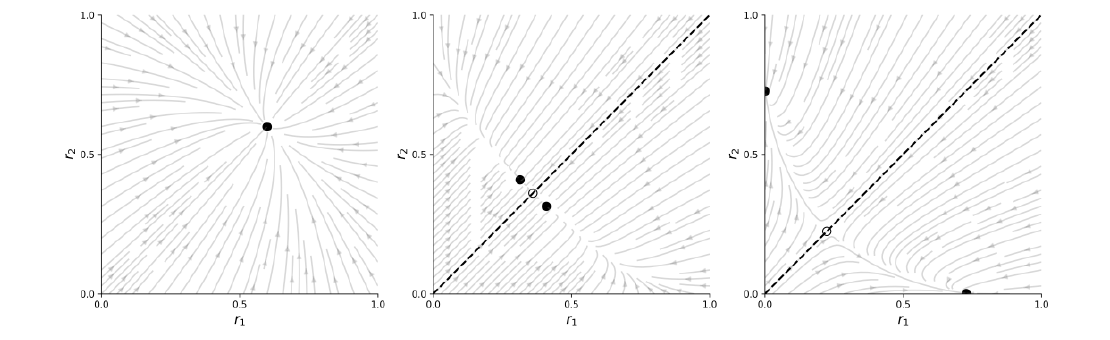
\includegraphics[width=0.97\linewidth]{mutual_inhibition_phase_portraits}}
\figcap{\src{LMLF Fig.\ 2.13}. Trajectories (grey) in the $(r_1,r_2)$ plane for $J=1$, $4.35$ and $10$ (left to right), with $\theta=0$, $\beta=1$, $\hext=1$. Full circles: stable fixed points; empty circles: unstable. Dashed: the separatrix $r_1=r_2$.
Left: everything flows to the homogeneous point $(0.60,0.60)$. Middle (just past $J_c$): the two winners sit close to the diagonal. Right: the winners are near the axes, $(0.73,0.002)$ and $(0.002,0.73)$.}
\end{center}

\begin{pitfall}[Typo in the book's caption]
The caption of \src{LMLF Fig.\ 2.13} reads ``$J=1,435,10$''. It means $J=1$, $4.35$, $10$. The middle value is just above the critical $J_c\approx4.33$, which is why its two stable fixed points are still close to the unstable homogeneous one ($r_1^*\approx0.31$ and $0.41$, around $0.36$).
\end{pitfall}

\begin{defn}[Basin of attraction]
The \term{basin of attraction} of an attractor is the set of all initial states whose trajectories converge to it.
\end{defn}

\begin{defn}[Separatrix]
A \term{separatrix} is a curve in state space that separates two basins of attraction. A trajectory that starts exactly on it never reaches either attractor (here it goes to the unstable fixed point).
\end{defn}

For mutual inhibition with equal inputs and $J>J_c$:
\begin{itemize}
  \item basin of $(r_1^*>r_2^*)$: all starts with $r_1>r_2$;
  \item basin of $(r_1^*<r_2^*)$: all starts with $r_1<r_2$;
  \item separatrix: the diagonal $r_1=r_2$. A start on it keeps $r_1=r_2$ forever (by symmetry) and slides to the unstable homogeneous point.
\end{itemize}
\hl{Whoever starts ahead wins}, however small the lead. This is the two-dimensional version of the autapse's watershed at $r=0.5$.

\begin{pitfall}[The diagonal is the separatrix only because of the symmetry]
That the separatrix is exactly $r_1=r_2$ relies on the two neurons being identical and getting identical input. With different inputs $h_1^{\text{ext}}\neq h_2^{\text{ext}}$ the symmetry is gone, and the boundary between the basins moves: the neuron with the stronger input can win even from a small deficit.
\end{pitfall}

\section{Decision making and perceptual bistability}

The book's interpretation \src{LMLF \S2.3.2}: let $r_1$ and $r_2$ be two \emph{populations} of neurons, each standing for one choice.
\begin{itemize}
  \item The external inputs $h_1^{\text{ext}}(t)$ and $h_2^{\text{ext}}(t)$ are the \textbf{evidence} for each option, arriving over time.
  \item The initial state is a prior \textbf{bias} towards one option.
  \item Mutual inhibition makes the populations compete. The network ends in one of the two asymmetric attractors: \hl{the decision}. Ending at $r_1^*>r_2^*$ means ``do action 1''.
\end{itemize}
Mutual inhibition between populations is considered a neural basis of binary decision making; the book returns to it in \S4.2.2.

\begin{defn}[Perceptual bistability]
\term{Perceptual bistability}: an ambiguous image has two interpretations, but at any moment we perceive only one of them, never a blend.
\end{defn}

\begin{center}
\fcolorbox{border}{white}{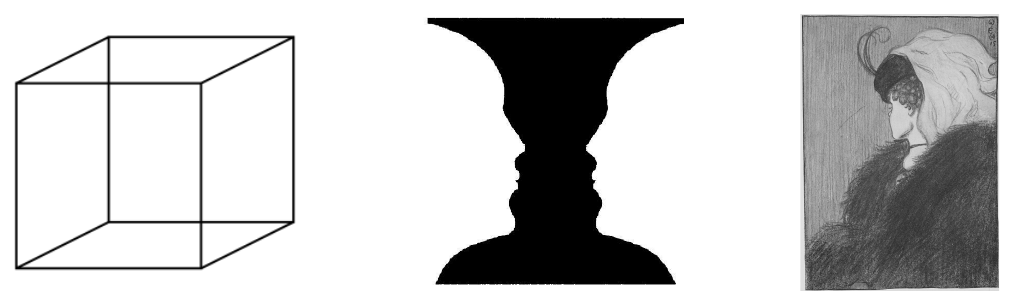
\includegraphics[width=0.85\linewidth]{perceptual_bistability}}
\figcap{\src{LMLF Fig.\ 2.14}. Left: the Necker cube (which face is in front?). Middle: Rubin's vase (a vase, or two faces in profile?). Right: ``My Wife and My Mother-in-Law'' (a young or an old woman?).}
\end{center}

The mutual-inhibition explanation: one population per percept; the ambiguous image drives both; inhibition lets only one stay active; which one depends on the initial state and on noise.

\begin{pitfall}[What the model does not explain]
Stare at the Necker cube long enough and the percept \emph{flips} every few seconds. Our model cannot do that: once in an attractor, it stays forever. Explaining the flips needs extra ingredients, such as slow \emph{adaptation} (the winner gets tired) and \emph{noise} \src{LMLF \S2.3.2}.
\end{pitfall}

% =================================================================
\section{Excitation and inhibition: the model}

So far the networks were purely excitatory (the autapse) or purely inhibitory (mutual inhibition). The minimal network with \emph{both} kinds has one excitatory neuron, E, and one inhibitory neuron, I \src{LMLF \S2.3.3}.

\begin{center}
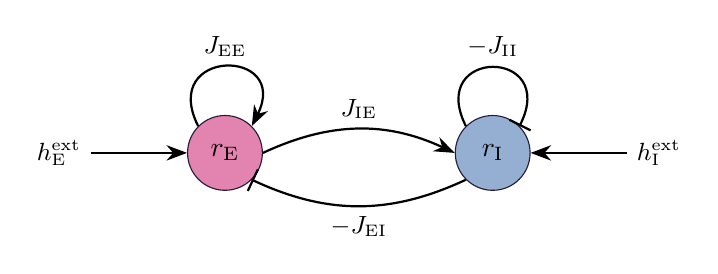
\begin{tikzpicture}
  \node[draw=ink,fill=ppink!60,circle,minimum size=0.95cm,font=\sffamily\bfseries] (E) at (0,0) {$r_\E$};
  \node[draw=ink,fill=pcyan!50,circle,minimum size=0.95cm,font=\sffamily\bfseries] (I) at (3.4,0) {$r_\I$};
  \draw[thick,->] (E.north west) .. controls +(-0.5,1.0) and +(0.5,1.0) .. (E.north east) node[pos=0.5,above,font=\small]{$J_{\E\E}$};
  \draw[thick,-{Bar[width=3mm]}] (I.north west) .. controls +(-0.5,1.0) and +(0.5,1.0) .. (I.north east) node[pos=0.5,above,font=\small]{$-J_{\I\I}$};
  \draw[thick,->] (E.east) to[bend left=25] node[above,font=\small]{$J_{\I\E}$} (I.west);
  \draw[thick,-{Bar[width=3mm]}] (I.south west) to[bend left=25] node[below,font=\small]{$-J_{\E\I}$} (E.south east);
  \draw[thick,->] (-1.7,0) node[left,font=\small]{$h_\E^{\text{ext}}$} -- (E.west);
  \draw[thick,->] (5.1,0) node[right,font=\small]{$h_\I^{\text{ext}}$} -- (I.east);
\end{tikzpicture}
\figcap{One excitatory and one inhibitory neuron, redrawn after \src{LMLF Fig.\ 2.15}. Arrowheads: excitation; bars: inhibition.}
\end{center}

The equations ($\tau=1$) \src{LMLF eq.\ 2.38--2.39}:
\[ \dot r_\E=-r_\E+g(h_\E),\qquad \dot r_\I=-r_\I+g(h_\I), \]
\[ h_\E=J_{\E\E}r_\E-J_{\E\I}r_\I+h_\E^{\text{ext}},\qquad h_\I=J_{\I\E}r_\E-J_{\I\I}r_\I+h_\I^{\text{ext}}. \]

\begin{itemize}
  \item $J_{\alpha\beta}>0$ is the synapse \hl{from $\beta$ to $\alpha$} (second index = source, as in Week 1). So $J_{\E\I}$ is the inhibition that I sends \emph{to} E.
  \item Excitatory or inhibitory is again the $\pm$ sign in front: E's synapses enter with $+$, I's with $-$ (Dale's principle, Week 1: a neuron is either excitatory or inhibitory for all its targets).
  \item Both external inputs are excitatory: $h_\E^{\text{ext}}>0$, $h_\I^{\text{ext}}>0$.
\end{itemize}

\begin{defn}[Threshold-linear activation (recap of Week 1)]
This time $g$ is the \term{threshold-linear} function: $g(h)=h$ for $h\ge0$ and $g(h)=0$ for $h<0$, i.e.\ $g(h)=\max(h,0)$. Below threshold the neuron is silent; above it the rate equals the input. There is no saturation from above.
\end{defn}

\begin{pitfall}[Reading $J_{\E\I}$ backwards]
$J_{\E\I}$ is \emph{not} ``from E to I''. The first index is the receiver. In $h_\E$ the inhibitory term is $-J_{\E\I}r_\I$: E receives from I. A quick check: every term in $h_\alpha$ has the form $J_{\alpha\beta}r_\beta$, with the source index $\beta$ appearing twice, next to each other.
\end{pitfall}

\section{The fixed point of the E--I network}

\subsection{Solving in the linear regime}

The model can do several things depending on its six parameters; the book follows only the regime where something new happens: oscillations.

\textbf{Step 1: drop the threshold.} As long as both inputs are positive, $g(h)=h$, and the dynamics are linear \src{LMLF eq.\ 2.40}:
\[ \dot{\vec r}=-\vec r+J\vec r+\vec h^{\text{ext}},\qquad J=\begin{pmatrix}J_{\E\E}&-J_{\E\I}\\J_{\I\E}&-J_{\I\I}\end{pmatrix},\quad \vec r=\begin{pmatrix}r_\E\\r_\I\end{pmatrix}. \]
(Here $J$ is the \emph{connectivity matrix}, with the signs included.)

\textbf{Step 2: set $\dot{\vec r}=0$.} $(I-J)\vec r^*=\vec h^{\text{ext}}$, so
\[ \vec r^*=(I-J)^{-1}\vec h^{\text{ext}}\qquad\text{\src{LMLF eq.\ 2.41}}. \]

\textbf{Step 3: invert the $2\times2$ matrix} (swap the diagonal, negate the off-diagonal, divide by the determinant):
\[ I-J=\begin{pmatrix}1-J_{\E\E}&J_{\E\I}\\-J_{\I\E}&1+J_{\I\I}\end{pmatrix},\qquad (I-J)^{-1}=\frac{1}{\det(I-J)}\begin{pmatrix}1+J_{\I\I}&-J_{\E\I}\\J_{\I\E}&1-J_{\E\E}\end{pmatrix}, \]
\[ \det(I-J)=(1-J_{\E\E})(1+J_{\I\I})+J_{\E\I}J_{\I\E}. \]

\textbf{Step 4: the assumption.} The book takes the E$\leftrightarrow$I loop to be strong compared with the self-connections \src{LMLF eq.\ 2.43}:
\[ J_{\E\I}J_{\I\E}>(J_{\E\E}-1)(1+J_{\I\I}), \]
which is exactly $\det(I-J)>0$.

\textbf{Step 5: is the solution allowed?} Step 1 assumed positive inputs, i.e.\ positive rates. Multiplying out,
\[ r_\E^*\propto(1+J_{\I\I})h_\E^{\text{ext}}-J_{\E\I}h_\I^{\text{ext}},\qquad r_\I^*\propto J_{\I\E}h_\E^{\text{ext}}+(1-J_{\E\E})h_\I^{\text{ext}}, \]
so both are positive when
\[ h_\E^{\text{ext}}>\frac{J_{\E\I}}{1+J_{\I\I}}\,h_\I^{\text{ext}}\qquad\text{and}\qquad h_\E^{\text{ext}}>\frac{J_{\E\E}-1}{J_{\I\E}}\,h_\I^{\text{ext}}. \]
The book's condition: the input to E must be strong enough compared with the input to I.

\begin{example}[The book's Fig.\ 2.16 parameters]
$J_{\E\E}=3$, $J_{\E\I}=4$, $J_{\I\E}=1$, $J_{\I\I}=0$, $h_\E^{\text{ext}}=1$, $h_\I^{\text{ext}}=0.2$.
\begin{enumerate}
  \item $I-J=\begin{pmatrix}-2&4\\-1&1\end{pmatrix}$, $\det(I-J)=(-2)(1)-(4)(-1)=2>0$ \checkmark{} (assumption: $4\cdot1=4>(3-1)(1)=2$).
  \item $(I-J)^{-1}=\tfrac12\begin{pmatrix}1&-4\\1&-2\end{pmatrix}$.
  \item $\vec r^*=\tfrac12\begin{pmatrix}1-0.8\\1-0.4\end{pmatrix}=\begin{pmatrix}0.1\\0.3\end{pmatrix}$.
  \item Check the inputs: $h_\E=3(0.1)-4(0.3)+1=0.1=r_\E^*$ \checkmark, $h_\I=1(0.1)+0.2=0.3=r_\I^*$ \checkmark. Both positive, so $g(h)=h$ was legitimate.
\end{enumerate}
\end{example}

\subsection{Are there other fixed points?}

With threshold-linear $g$, a neuron at a fixed point is either active ($r^*=h^*>0$) or silent ($r^*=0$, $h^*\le0$). That gives four cases \src{LMLF \S2.3.3}:
\begin{enumerate}
  \item \textbf{Both active.} The solution above; unique, because $I-J$ is invertible.
  \item \textbf{Both silent.} Then the only input is the external drive, which is positive, so both would fire. Impossible.
  \item \textbf{E active, I silent.} I's input is $J_{\I\E}r_\E^*+h_\I^{\text{ext}}>0$, so I would fire. Impossible.
  \item \textbf{E silent, I active.} Then $r_\I^*=h_\I^{\text{ext}}/(1+J_{\I\I})$, and E silent requires $h_\E=-J_{\E\I}r_\I^*+h_\E^{\text{ext}}<0$, i.e.\ $h_\E^{\text{ext}}<\frac{J_{\E\I}}{1+J_{\I\I}}h_\I^{\text{ext}}$. That contradicts Step 5. Impossible.
\end{enumerate}
\hl{So there is exactly one fixed point, with both neurons active.} (Fig.\ 2.16 numbers, case 4: it would need $1<4\cdot0.2=0.8$, false.)

\section{Stability of the E--I fixed point}

\subsection{Trace, determinant and spirals}

Near the fixed point both inputs are positive, so the dynamics are exactly the linear ones of Step 1, and the Jacobian is read off directly \src{LMLF eq.\ 2.44}:
\[ M=-I+J=\begin{pmatrix}-1+J_{\E\E}&-J_{\E\I}\\J_{\I\E}&-1-J_{\I\I}\end{pmatrix},\qquad \Tr M=J_{\E\E}-J_{\I\I}-2,\qquad \det M=\det(I-J). \]
($M=-(I-J)$, and for a $2\times2$ matrix $\det(-A)=(-1)^2\det A=\det A$.)

Recall Week 1: the eigenvalues satisfy $\mu_1+\mu_2=\Tr M$ and $\mu_1\mu_2=\det M$, and
\[ \mu_{1,2}=\frac{\Tr M\pm\sqrt{(\Tr M)^2-4\det M}}{2}. \]
\begin{itemize}
  \item If $(\Tr M)^2<4\det M$, the eigenvalues are complex conjugates $\alpha\pm i\omega$ with real part $\alpha=\Tr M/2$. The trajectories \textbf{spiral} (Week 2 Part C): inwards if $\Tr M<0$, outwards if $\Tr M>0$.
  \item In that case stability is decided by the trace alone:
\end{itemize}

\begin{formula}[Stability of the E--I fixed point (complex eigenvalues)]
\[ \Tr M<0\iff J_{\E\E}<2+J_{\I\I}:\ \text{stable spiral};\qquad J_{\E\E}>2+J_{\I\I}:\ \text{unstable spiral}. \]
Self-excitation of E destabilizes; self-inhibition of I stabilizes.
\end{formula}

\begin{pitfall}[$\det M>0$ does \emph{not} make the eigenvalues complex]
The book says that $\det M>0$ ``implies that the two eigenvalues of $M$ are complex conjugate''. That is not right. $\det M>0$ only says the eigenvalues have the same sign (or are a complex pair). They are complex iff $(\Tr M)^2<4\det M$, which works out to
\[ (J_{\E\E}+J_{\I\I})^2<4J_{\E\I}J_{\I\E}\qquad\text{i.e.}\qquad J_{\E\I}J_{\I\E}>\tfrac14(J_{\E\E}+J_{\I\I})^2 : \]
the E$\leftrightarrow$I loop must beat the self-connections by a margin.
\textbf{Counterexample}: $J_{\E\E}=3$, $J_{\I\I}=0$, $J_{\I\E}=1$, $J_{\E\I}=2.1$. The book's assumption holds ($2.1>2$), and $\det M=0.1>0$. But $\Tr M=1$ and $(\Tr M)^2-4\det M=0.6>0$: the eigenvalues are \emph{real}, $0.887$ and $0.113$. An unstable \emph{node}: trajectories leave without spiralling.
The book's conclusions hold for its Fig.\ 2.16 example, where $4J_{\E\I}J_{\I\E}=16>9=(J_{\E\E}+J_{\I\I})^2$.
\end{pitfall}

\begin{example}[Turning up $J_{\E\E}$ ($J_{\E\I}=4$, $J_{\I\E}=1$, $J_{\I\I}=0$, $h_\E^{\text{ext}}=1$, $h_\I^{\text{ext}}=0.2$)]
\begin{center}
\renewcommand{\arraystretch}{1.25}
\begin{tabular}{c|cc|c|c|l}
$J_{\E\E}$ & $\Tr M$ & $\det M$ & eigenvalues & $\vec r^*$ & behaviour\\\hline
1.5 & $-0.5$ & 3.5 & $-0.25\pm1.85i$ & $(0.057,0.257)$ & stable spiral\\
2 & $0$ & 3 & $\pm1.73i$ & $(0.067,0.267)$ & borderline\\
3 & $+1$ & 2 & $0.5\pm1.32i$ & $(0.1,0.3)$ & unstable spiral\\
\end{tabular}
\end{center}
At $J_{\E\E}=1.5$ a perturbation spirals back in, with damped oscillations of period $2\pi/1.85\approx3.4$ (units of $\tau$). At $J_{\E\E}=3$ it spirals out.
\end{example}

\begin{defn}[Hopf bifurcation]
A \term{Hopf bifurcation} happens when a fixed point loses stability because a \hl{pair of complex-conjugate eigenvalues crosses the imaginary axis}: the real part goes from negative to positive while the imaginary part stays non-zero.
Here that happens at $J_{\E\E}=2+J_{\I\I}$. It is the third bifurcation of the course: saddle-node (fixed points merge and vanish), pitchfork (one becomes unstable and two are born), Hopf (a spiral turns from inward to outward).
\end{defn}

\subsection{Link to TA session 2}

Exam 2015 Q2 (Week 2 Part C) was the same idea with $\tanh$ instead of threshold-linear $g$ and with the fixed point at $(0,0)$. There $\Tr=-2$ was fixed, so the spiral was always stable; oscillations needed $K>J$, the loop beating the self-coupling.
The book's model adds what the exam left out: the trace can turn positive, the spiral can turn outward, and then something new must happen.

\section{Limit cycles: the network oscillates}\label{sec:limitcycle}

\subsection{What happens after the spiral leaves?}

When $J_{\E\E}>2+J_{\I\I}$, the only fixed point is unstable, and trajectories spiral away from it. Where do they go?
\begin{itemize}
  \item If $g$ were linear everywhere, the linear analysis would hold for every $\vec r$: the spiral would grow forever and the rates would diverge.
  \item The threshold stops this. Step by step \src{LMLF \S2.3.3}:
  \begin{enumerate}
    \item As the spiral grows, I's rate swings high, and E's input $h_\E=J_{\E\E}r_\E-J_{\E\I}r_\I+h_\E^{\text{ext}}$ becomes \emph{negative}.
    \item Then $g(h_\E)=0$: E's rate decays exponentially towards $0$. The outward push is switched off.
    \item With E low, I loses its excitatory drive, and its rate falls.
    \item With I low, E's input becomes positive again, and E's rate climbs.
    \item With both inputs positive, the outward spiral resumes. Back to step 1.
  \end{enumerate}
\end{itemize}
Outward push near the fixed point plus inward pull far from it: the trajectories settle on a closed loop in between.

\begin{defn}[Limit cycle]
A \term{limit cycle} is a closed trajectory that is \textbf{isolated}: nearby trajectories are not closed, but spiral towards it (a \term{stable} limit cycle) or away from it (unstable).
A stable limit cycle is an \hl{attractor}. Along it the rates repeat periodically: the network \textbf{oscillates}.
\end{defn}

\begin{pitfall}[A closed orbit is not automatically a limit cycle]
A frictionless pendulum (a harmonic oscillator) also has closed periodic orbits, but a whole family of them: start a bit further out and you stay on a bigger orbit forever. None of them attracts anything, so none is a limit cycle.
A limit cycle has a \emph{preferred} amplitude, reached from any start nearby. The borderline case $\Tr M=0$ (purely imaginary eigenvalues, the middle row above) is exactly such a pendulum near the fixed point: a family of closed orbits, none of them attracting.
\end{pitfall}

\begin{center}
\fcolorbox{border}{white}{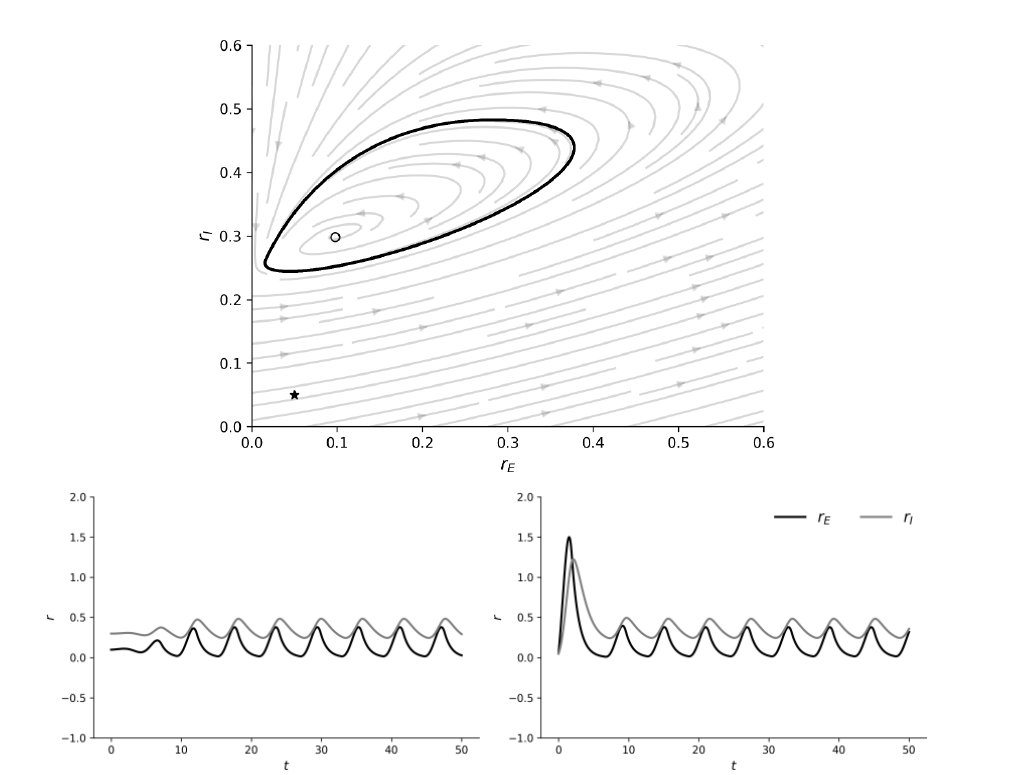
\includegraphics[width=0.78\linewidth]{ei_limit_cycle}}
\figcap{\src{LMLF Fig.\ 2.16}; $J_{\E\E}=3$, $J_{\E\I}=4$, $J_{\I\E}=1$, $J_{\I\I}=0$, $h_\E^{\text{ext}}=1$, $h_\I^{\text{ext}}=0.2$.
Top: trajectories in the $(r_\E,r_\I)$ plane; thick black curve: the limit cycle; open circle: the unstable fixed point $(0.1,0.3)$; star: a start far outside, $(0.05,0.05)$.
Bottom: $r_\E$ (black) and $r_\I$ (grey) against time, starting near the fixed point (left) and at the star (right). Both end on the same oscillation.}
\end{center}

\begin{example}[The limit cycle in numbers (Fig.\ 2.16 parameters, by simulation)]
\begin{itemize}
  \item Near the fixed point the linear analysis gives $\mu=0.5\pm1.32i$: the spiral grows by $e^{0.5t}$ and turns with angular frequency $1.32$, i.e.\ period $2\pi/1.32\approx4.8$.
  \item On the limit cycle: $r_\E$ swings between $0.015$ and $0.38$, $r_\I$ between $0.24$ and $0.48$. The period is $\approx5.9$ (in units of $\tau$; with $\tau=10$\,ms about $59$\,ms, i.e.\ roughly $17$\,Hz).
  \item Starting near $(0.1,0.3)$ or at $(0.05,0.05)$ (where $r_\E$ first overshoots to $1.5$) gives the \emph{same} final amplitude and period: that is what ``attractor'' means.
  \item The period on the cycle ($5.9$) is longer than the linear one ($4.8$): part of each cycle is spent with E silent, outside the linear regime.
\end{itemize}
\end{example}

\begin{pitfall}[What we cannot compute here]
Finding the limit cycle exactly, and proving it is stable, is much harder than finding fixed points; the book leaves it out. (The method it sketches: in each region where the signs of $h_\E$, $h_\I$ are fixed the equations are linear and solvable; glue the pieces so that the end state in one region is the start state in the next.) Here we rely on simulation.
\end{pitfall}

\subsection{Why it oscillates: delayed negative feedback}

Read the cycle in terms of the neurons:
\begin{enumerate}
  \item E rises $\Rightarrow$ it drives I up.
  \item I high $\Rightarrow$ it inhibits E, which falls.
  \item E low $\Rightarrow$ I loses drive and falls.
  \item I low $\Rightarrow$ E is released and rises again.
\end{enumerate}
E acts on itself through I with a minus sign: \textbf{negative feedback}.

\begin{intuition}[Why does an inhibitory autapse not oscillate?]
An inhibitory autapse is negative feedback too. It is just the homogeneous mode of mutual inhibition (\S\ref{sec:disinhibition}), with eigenvalue $\mu_\parallel=-(1+a)<0$: always stable, never oscillating.
The difference is \hl{delay}. In the autapse, the neuron feels its own inhibition at once. In the E--I loop, a change of E reaches E again only after I has had time to respond. By then E has already moved on, so the correction arrives late and overshoots.
\end{intuition}

\begin{example}[The hotel shower \src{LMLF \S2.3.3}]
You turn on the hot water; it comes out cold, because hot water takes a few seconds to reach the shower head. You turn it up. Still cold. Up more. Now it is pleasant, so you step in, and seconds later it is scalding, because all your earlier turns are arriving. You turn it back, still too hot, back more, and suddenly it is freezing.
The rule (hot when cold, cold when hot) is negative feedback; the pipe is the delay. Together they make the temperature \textbf{oscillate} around the one you want, an unstable target.
\end{example}

\begin{intuition}[Why this matters in the brain]
Rhythmic activity is everywhere in the nervous system: circuits that generate walking, swimming, breathing and chewing; rhythms thought to help encode sensory information and to support spatial navigation; and brain rhythms recorded by EEG, used clinically to diagnose epilepsy and sleep disorders.
The E--I loop is one of the simplest mechanisms that generates them.
\end{intuition}

\section{Summary: three networks}

\begin{center}\small
\renewcommand{\arraystretch}{1.35}
\begin{tabular}{>{\columncolor{border}\raggedright\arraybackslash}m{2.6cm} >{\raggedright\arraybackslash}m{3.2cm} >{\raggedright\arraybackslash}m{3.5cm} >{\raggedright\arraybackslash}m{3.6cm}}
\thd{NETWORK} & \cellcolor{border}\thd{FEEDBACK} & \cellcolor{border}\thd{INSTABILITY} & \cellcolor{border}\thd{ATTRACTORS / FUNCTION}\\
\rowcolor{surface}\cellcolor{border}\color{surface}Excitatory autapse & positive (self-excitation) & $Jg'>1$; saddle-node in $\hext$ & two stable rates: \textbf{memory}\\
\rowcolor{surface2}\cellcolor{border}\color{surface}Mutual inhibition & positive (disinhibition loop) & $a=Jg'(h^*)>1$; pitchfork in $J$ & one neuron wins: \textbf{decision}\\
\rowcolor{surface}\cellcolor{border}\color{surface}E--I pair & delayed negative (E$\to$I$\to$E) & $J_{\E\E}>2+J_{\I\I}$; Hopf & limit cycle: \textbf{oscillation}\\
\end{tabular}
\end{center}

\begin{intuition}[The method, every time]
\begin{enumerate}
  \item Find the fixed points (graphically, by symmetry, or by solving a linear system).
  \item Linearize: the Jacobian $M$.
  \item Eigenvalues of $M$: all real parts negative $\Rightarrow$ stable. For $2\times2$, use trace and determinant.
  \item If a fixed point becomes unstable, ask what the nonlinearity (saturation, threshold) does: new fixed points (bistability) or a limit cycle (oscillation).
\end{enumerate}
\end{intuition}

% =================================================================
\parttitle{WEEK 03}{Practice Problems and Summary}
% =================================================================

\section{Practice problems with full solutions}

\begin{example}[P1: Can it be bistable at all?]
An excitatory autapse with (a) $\beta=2$, $J=1$; (b) $\beta=20$, $J=0.15$; (c) $\beta=8$, $J=1$. For which can a suitable $\hext$ give two stable states?

\textbf{Solution.} Test $\beta J/4>1$: (a) $0.5$, no. (b) $0.75$, no. (c) $2$, yes. In (a) and (b) the S-curve is everywhere flatter than the identity line, so it crosses it once whatever $\hext$ is.
\end{example}

\begin{example}[P2: Writing a bit]
With $\theta=0$, $\beta=20$, $J=1$, $\tau=10$\,ms, the neuron rests at the low state with $\hext=-0.5$. You can pulse $\hext$ to $0$. A 5\,ms pulse brings $r$ to $0.36$, a 15\,ms pulse to $0.76$. Which pulse stores a ``1''? Why does setting $\hext=-0.3$ forever not count as memory?

\textbf{Solution.} Only the 15\,ms pulse: $0.76$ is above the unstable fixed point $0.5$ of $\hext=-0.5$, so the rate continues to the high state; $0.36$ is below it and decays back. Memory means the state persists \emph{after} the input returns to its baseline;
a permanent change of $\hext$ is just a different input, not a stored bit.
\end{example}

\begin{example}[P3: Half-stable]
At the bifurcation point $\hext=-0.197$ ($\beta=20$, $J=1$), $r^*=0.053$. Is $g''(h^*)$ positive or negative, and from which side is the fixed point approached?

\textbf{Solution.} $g''=\beta^2g(1-g)(1-2g)$ with $g=0.053<0.5$, so $g''>0$. Then $\tau\dot{\dr} = \tfrac12J^2g''\dr^2>0$ on both sides: $r$ increases. From below ($\dr<0$) it moves up towards $r^*$; from above it moves away, up towards the high state.
Half-stable, approached from the left.
\end{example}

\begin{example}[P4: Jacobian and modes]
Mutual inhibition with $\theta=0$, $\beta=1$, $\hext=1$, $J=3$; the homogeneous fixed point is $r^*=0.4288$. Write the Jacobian, its eigenvectors and eigenvalues, and decide stability.

\textbf{Solution.}
\begin{enumerate}
  \item $a=\beta Jr^*(1-r^*)=3\cdot0.4288\cdot0.5712=0.735$.
  \item $M=\begin{pmatrix}-1&-0.735\\-0.735&-1\end{pmatrix}$.
  \item Equal row sums: $(1,1)$ with $\mu_\parallel=-1.735$. Symmetric, so the other is $(1,-1)$ with $\mu_\perp=-(1-0.735)=-0.265$.
  \item Both negative: stable. (Check: $\mu_\parallel+\mu_\perp=-2=\Tr M$, $\mu_\parallel\mu_\perp=0.460=1-a^2=\det M$ \checkmark.)
\end{enumerate}
\end{example}

\begin{example}[P5: Fixed point or not?]
Same network with $J=5$. (a) Show that $(0.599,0.120)$ is a fixed point. (b) The homogeneous fixed point is $r^*=0.336$. Is it stable?

\textbf{Solution.} (a) $g(-5\cdot0.120+1)=g(0.4)=0.599$ and $g(-5\cdot0.599+1)=g(-1.995)=0.120$ \checkmark.
(b) $a=5\cdot0.336\cdot0.664=1.116>1$, so $\mu_\perp=+0.116>0$: unstable along $(1,-1)$. The asymmetric fixed points are where the network goes.
\end{example}

\begin{example}[P6: Which mode survives?]
In P4, start at $\vec{\dr}(0)=(0.02,0)$. Find $\dr_1$ and $\dr_2$ at $t=2$. Which pattern remains at late times?

\textbf{Solution.} $\dr_\pm(0)=0.02$. At $t=2$: $\dr_+=0.02e^{-3.47}=0.0006$, $\dr_-=0.02e^{-0.53}=0.0118$.
$\dr_1=\tfrac12(0.0006+0.0118)=0.0062$, $\dr_2=\tfrac12(0.0006-0.0118)=-0.0056$.
The homogeneous mode decays $6.5$ times faster ($1.735/0.265$), so at late times the perturbation is a pure difference, $\dr_1\approx-\dr_2$, slowly decaying.
\end{example}

\begin{example}[P7: Never unstable below $J=4$]
For mutual inhibition with $\beta=1$, show that the homogeneous fixed point is stable for every $J<4$, whatever $\hext$ is.

\textbf{Solution.} $a=Jr^*(1-r^*)$, and $r(1-r)\le\tfrac14$ for every $r$ (maximum at $r=\tfrac12$). So $a\le J/4<1$ when $J<4$, and $\mu_\perp=-(1-a)<0$, $\mu_\parallel<0$. (With the book's $\hext=1$ the actual threshold is $J_c\approx4.33$, consistent with the bound.)
\end{example}

\begin{example}[P8: Who wins?]
Mutual inhibition with $J=10$ ($\beta=1$, $\hext=1$). The network starts at (a) $(0.20,0.50)$; (b) $(0.50,0.49)$; (c) $(0.30,0.30)$. Where does it end?

\textbf{Solution.} The separatrix is $r_1=r_2$. (a) $r_2>r_1$: ends at $(0.0019,0.727)$. (b) $r_1>r_2$, however slightly: ends at $(0.727,0.0019)$. (c) On the separatrix: stays on the diagonal and goes to the unstable homogeneous point $(0.224,0.224)$; in practice any noise tips it to one side.
\end{example}

\begin{example}[P9: An E--I fixed point]
$J_{\E\E}=1.5$, $J_{\E\I}=4$, $J_{\I\E}=1$, $J_{\I\I}=0$, $h_\E^{\text{ext}}=1$, $h_\I^{\text{ext}}=0.2$. Find $\vec r^*$, check it is valid, and classify it.

\textbf{Solution.}
\begin{enumerate}
  \item $I-J=\begin{pmatrix}-0.5&4\\-1&1\end{pmatrix}$, $\det=-0.5+4=3.5$, $(I-J)^{-1}=\tfrac{1}{3.5}\begin{pmatrix}1&-4\\1&-0.5\end{pmatrix}$.
  \item $\vec r^*=\tfrac1{3.5}(1-0.8,\;1-0.1)=(0.057,\,0.257)$. Both positive \checkmark.
  \item $M=\begin{pmatrix}0.5&-4\\1&-1\end{pmatrix}$: $\Tr M=-0.5$, $\det M=3.5$, $(\Tr M)^2-4\det M=0.25-14<0$: complex.
  \item $\mu=-0.25\pm1.85i$: a \textbf{stable spiral}. Perturbations die out in damped oscillations with period $2\pi/1.85\approx3.4$.
\end{enumerate}
\end{example}

\begin{example}[P10: Spiral or node?]
$J_{\E\E}=3$, $J_{\E\I}=2.1$, $J_{\I\E}=1$, $J_{\I\I}=0$. Does the fixed point spiral?

\textbf{Solution.} $M=\begin{pmatrix}2&-2.1\\1&-1\end{pmatrix}$, $\Tr M=1$, $\det M=-2+2.1=0.1>0$. Discriminant $1-0.4=0.6>0$: real eigenvalues $\tfrac12(1\pm\sqrt{0.6})=0.887,\ 0.113$. Both positive: an \textbf{unstable node}, no spiralling, although $\det M>0$.
The complex condition $J_{\E\I}J_{\I\E}>\frac14(J_{\E\E}+J_{\I\I})^2$ reads $2.1>2.25$: false.
\end{example}

\begin{example}[P11: Where is the Hopf point?]
With $J_{\I\I}=0.5$ (other parameters as in Fig.\ 2.16, eigenvalues complex), for which $J_{\E\E}$ does the fixed point become unstable?

\textbf{Solution.} $\Tr M=J_{\E\E}-J_{\I\I}-2=J_{\E\E}-2.5$. Unstable iff $J_{\E\E}>2.5$. Self-inhibition of I moves the Hopf point up by $J_{\I\I}$.
(Check complex at $J_{\E\E}=2.5$: $4J_{\E\I}J_{\I\E}=16>(2.5+0.5)^2=9$ \checkmark.)
\end{example}

\begin{example}[P12: Concepts]
(a) Why can the homogeneous equation of mutual inhibition never have three solutions? (b) Why does the E--I network oscillate but an inhibitory autapse does not? (c) Why does the E--I rate not diverge when the fixed point is unstable?

\textbf{Solution.} (a) $r$ is increasing and $g(-Jr+\hext)$ is decreasing: they cross once. (b) Delay: in the loop, E's change returns through I only after I responds, so the correction overshoots; the autapse's negative feedback is instantaneous and just damps ($\mu_\parallel<0$).
(c) The threshold: when $h_\E<0$ the outward spiral is switched off and E decays to $0$, pulling the trajectory back. Push near the fixed point, pull far from it: a stable limit cycle.
\end{example}

\section{Cheat sheet}

\begin{formula}[Bistability and memory]
\begin{itemize}
  \item \textbf{Attractor}: region all nearby trajectories go to. \textbf{Bistable}: two stable fixed points, an unstable one between them as the watershed.
  \item \textbf{Memory}: a brief pulse of $\hext$ past a bifurcation point flips the state, which persists after the pulse (the state depends on history).
  \item \textbf{Ingredients}: positive feedback ($\beta J/4>1$) and saturation.
  \item $\lambda=1$: second order, $\tau\dot{\dr} = \tfrac12J^2g''\dr^2$: \textbf{half-stable}, hyperbolic (slow) approach.
\end{itemize}
\end{formula}

\begin{formula}[Mutual inhibition]
\begin{itemize}
  \item $\dot r_1=-r_1+g(-Jr_2+\hext)$, $\dot r_2=-r_2+g(-Jr_1+\hext)$, $J>0$.
  \item Homogeneous fixed point $r^*=g(-Jr^*+\hext)$: always exactly one (rising line vs.\ falling curve).
  \item \textbf{Jacobian} $M_{ij}=\partial F_i/\partial r_j$: $M=\begin{pmatrix}-1&-a\\-a&-1\end{pmatrix}$, $a=Jg'(h^*)=\beta Jr^*(1-r^*)$.
  \item Modes: $(1,1)$, $\mu_\parallel=-(1+a)$, always stable; $(1,-1)$, $\mu_\perp=-(1-a)$, unstable iff $a>1$.
  \item $\dr_{1,2}=\tfrac12[\dr_+(0)e^{-(1+a)t}\pm\dr_-(0)e^{-(1-a)t}]$.
  \item $a>1$: \textbf{pitchfork}, symmetry breaking, two stable winner states. Positive feedback = \textbf{disinhibition}.
  \item Book values $\beta=1$, $\hext=1$: $J_c\approx4.33$; $J=5$: $(0.599,0.120)$; $J=10$: $(0.727,0.0019)$.
  \item Basins $r_1>r_2$ and $r_1<r_2$; separatrix $r_1=r_2$. Decision making; perceptual bistability (flips need adaptation + noise).
\end{itemize}
\end{formula}

\begin{formula}[Excitation and inhibition]
\begin{itemize}
  \item $h_\E=J_{\E\E}r_\E-J_{\E\I}r_\I+h_\E^{\text{ext}}$, $h_\I=J_{\I\E}r_\E-J_{\I\I}r_\I+h_\I^{\text{ext}}$; $J_{\alpha\beta}$: from $\beta$ to $\alpha$; $g(h)=\max(h,0)$.
  \item Fixed point $\vec r^*=(I-J)^{-1}\vec h^{\text{ext}}$, $\det(I-J)=(1-J_{\E\E})(1+J_{\I\I})+J_{\E\I}J_{\I\E}>0$; unique if $h_\E^{\text{ext}}$ is large enough relative to $h_\I^{\text{ext}}$.
  \item $M=-I+J$, $\Tr M=J_{\E\E}-J_{\I\I}-2$, $\det M=\det(I-J)$.
  \item Complex iff $J_{\E\I}J_{\I\E}>\frac14(J_{\E\E}+J_{\I\I})^2$ ($\det>0$ is \emph{not} enough). Then stable iff $J_{\E\E}<2+J_{\I\I}$.
  \item \textbf{Hopf}: complex pair crosses the imaginary axis. Beyond it: stable \textbf{limit cycle} (isolated closed orbit, an attractor), kept finite by the threshold.
  \item Fig.\ 2.16: $\vec r^*=(0.1,0.3)$, $\mu=0.5\pm1.32i$, cycle period $\approx5.9\tau$.
  \item Mechanism: \textbf{delayed negative feedback} (the hotel shower).
\end{itemize}
\end{formula}

\end{document}
